\documentclass[12pt,a4paper]{article}

% =================================================
% Font (XeLaTeX or LuaLaTeX REQUIRED)
% =================================================
\usepackage{fontspec}
\setmainfont{Open Sans}

\usepackage{listings}
\usepackage{xcolor}
\usepackage{subcaption}

\lstset{
    language=Python,
    basicstyle=\ttfamily\small,
    keywordstyle=\color{blue},
    stringstyle=\color{red},
    commentstyle=\color{gray},
    showstringspaces=false,
    breaklines=true,
    frame=single
}

% =================================================
% Math and symbols
% =================================================
\usepackage{amsmath,amssymb,amsfonts}

% =================================================
% Graphics and floats
% =================================================
\usepackage{graphicx}
\usepackage{float}
\usepackage{placeins}

\usepackage{hanging}
\usepackage{ragged2e}

% =================================================
% Tables
% =================================================
\usepackage{booktabs}
\usepackage{multirow}
\usepackage{array}

% =================================================
% Lists and layout
% =================================================
\usepackage{enumitem}
\usepackage{geometry}
\geometry{margin=1in}

% =================================================
% Algorithms
% =================================================
\usepackage{algorithm}
\usepackage{algpseudocode}

\floatname{algorithm}{Algorithm}

\newcommand{\kw}[1]{\textbf{#1}}
\newcommand{\ty}[1]{\texttt{#1}}
\newcommand{\cmt}[1]{\textcolor{gray}{$\triangleright$ \textit{#1}}}
\algrenewcommand{\algorithmiccomment}[1]{\hfill\cmt{#1}}

% =================================================
% TOC customization
% =================================================
\usepackage[titles]{tocloft}
\renewcommand{\cftsecleader}{\cftdotfill{\cftdotsep}}

% =================================================
% Citations
% =================================================
\usepackage{cite}

% =================================================
% Hyperlinks (no colors, no boxes)
% =================================================
\usepackage[hidelinks]{hyperref}

% =================================================
% PDF imports
% =================================================
\usepackage{pdfpages}


\title{
\textbf{Adaptive Multi-LLM Agentic RAG with Dynamic Task Routing and Retrieval Planning}
}


\begin{document}

\maketitle

\begin{abstract}
The rapid growth of large language models (LLMs) creates both opportunities and challenges for scalable conversational AI. Most current systems rely on monolithic pipelines that apply uniform inference strategies, leading to inefficiencies, increased hallucination risk, and underutilisation of diverse model strengths. This paper presents an Adaptive Multi-LLM Agentic Retrieval-Augmented Generation (RAG) system that addresses these limitations through dynamic task routing, specialist model selection, and selective retrieval. Built on LangGraph, the system integrates ten heterogeneous open-weight and API-based models. A central orchestration layer classifies queries by task type and complexity, routing them to one of three execution paths: direct inference, retrieval-augmented generation using a ChromaDB vector store, or agentic multi-step execution with web search and computational tools. State persistence is managed via a MySQL-backed checkpointing mechanism, enabling resumable multi-turn interactions. The system is evaluated on the HotpotQA and MuSiQue multi-hop question-answering benchmarks using metrics including Exact Match, F1 Score, Retrieval Precision, Routing Accuracy, and response latency. Results demonstrate that adaptive multi-LLM orchestration outperforms monolithic baselines in both accuracy and computational efficiency.
\end{abstract}

\noindent \textbf{Index Terms:} Large Language Models, Retrieval-Augmented Generation, Multi-Agent Systems, Dynamic Routing, LangGraph, Question Answering.

\vspace{0.5cm}
\hrule
\vspace{0.5cm}

\section{Introduction}

Recent advances in large language models (LLMs) have transformed artificial intelligence, enabling systems capable of sophisticated reasoning, code generation, and instruction following \cite{brown2020language, wei2022chain}. Models such as GPT-4, LLaMA, Mistral, and Gemini have democratised access to generative capabilities and spurred interest in production-grade AI assistants across diverse domains \cite{touvron2023llama, jiang2023mistral, team2024gemini}.

Despite these advances, most deployed systems rely on monolithic pipelines in which a single model handles all queries uniformly, regardless of task complexity or retrieval requirements \cite{singh2025agentic}. This is inherently suboptimal: simple queries incur unnecessary retrieval overhead, while complex multi-hop tasks may fail without structured external knowledge. Retrieval-Augmented Generation (RAG) mitigates hallucinations in knowledge-intensive settings \cite{lewis2020retrieval}, yet indiscriminate retrieval introduces noise and latency for queries the model can already answer accurately \cite{shi2023large, asai2023self}. Agentic extensions further compound this by imposing execution overhead regardless of query complexity \cite{yao2023react}.

This paper proposes an Adaptive Multi-LLM Agentic RAG system addressing these limitations through three innovations: (1) an intent-aware query router that classifies queries by task type and complexity; (2) a specialist model orchestration layer selecting dynamically from ten heterogeneous LLMs; and (3) a retrieval necessity predictor that activates document retrieval only when beneficial. These components form a cost-aware, quality-preserving pipeline implemented using the LangGraph stateful orchestration framework \cite{zhao2024langgraph}.

\section{System Architecture}

\subsection{Overview}

The proposed system is designed around a modular, graph-based orchestration architecture implemented using LangGraph. The high-level architectural philosophy is one of selective activation: components are only invoked when their contribution is predicted to improve the final response quality. This contrasts with always-on architectures where retrieval, agentic reasoning, and complex prompting are applied uniformly regardless of query requirements.

\begin{figure}[htbp]
    \centering
    \includegraphics[width=0.9\linewidth]{../assets/architecture_diagram.png}
    \caption{High-level architecture of the Adaptive Multi-LLM Agentic RAG system.}
    \label{fig:arch_overview}
\end{figure}

The architecture comprises five principal layers, as depicted in Figure~\ref{fig:arch_overview}. The User Interface layer provides the Streamlit-based web frontend and session management functionality. The Persistence layer manages conversation state through MySQL-backed LangGraph checkpointing. The Core Orchestration layer implements the LangGraph StateGraph with conditional routing edges. The Execution layer hosts the three processing nodes (direct, RAG, agent) and the model orchestrator. The Model Pool layer provides access to the ten deployed LLMs through the Groq inference API.

\subsection{LangGraph State Management}

The system's execution state is represented as a typed \texttt{ChatState} dictionary managed by LangGraph's \texttt{StateGraph}. The state schema, defined in \texttt{app/models/chat\_state.py}, encapsulates all information required for a single conversation turn, as formalised in Algorithm~\ref{alg:chatstate}.

\begin{algorithm}[H]
\caption{ChatState TypedDict definition managing conversation context and routing metadata.}
\label{alg:chatstate}
\begin{algorithmic}[1]
  \State \kw{TypedDict} \ty{ChatState}:
  \State \hspace{\algorithmicindent}
         \ty{messages}     : \ty{Annotated[list[BaseMessage], add\_messages]}
  \State \hspace{\algorithmicindent}
         \ty{model}        : \ty{str}
  \State \hspace{\algorithmicindent}
         \ty{routing\_info}: \ty{Optional[dict]}
  \State \hspace{\algorithmicindent}
         \ty{rag\_context} : \ty{Optional[str]}
  \State \hspace{\algorithmicindent}
         \ty{route}        : \ty{Optional[str]}
\end{algorithmic}
\end{algorithm}

The LangGraph \texttt{StateGraph} is constructed with the \texttt{ChatState} as its state type, and four nodes are registered: \texttt{router\_node}, \texttt{direct\_node}, \texttt{rag\_node}, and \texttt{agent\_node}. The graph topology is defined as: \texttt{START} $\rightarrow$ \texttt{router\_node} $\rightarrow$ \{\texttt{direct\_node} $|$ \texttt{rag\_node} $|$ \texttt{agent\_node}\} $\rightarrow$ \texttt{END}.

\subsection{Deployed Language Models}

A central contribution of this paper is the integration and evaluation of ten heterogeneous language models within a unified orchestration framework. Table~\ref{tab:models} summarises the key characteristics of each deployed model.

\begin{table}[htbp]
\centering
\caption{Deployed language models with their primary specialisations and context window sizes.}
\label{tab:models}
\begin{tabular}{|l|l|c|p{3.5cm}|}
\hline
\textbf{Model Key} & \textbf{Model Name} & \textbf{Context (tokens)} & \textbf{Primary Specialisation} \\
\hline
deepseek\_r1 & DeepSeek-R1 & 8,000 & Advanced multi-step reasoning \\
\hline
falcon3 & Falcon-3 & 3,000 & General language understanding \\
\hline
gemma3\_270m & Gemma-3-270M & 2,000 & Lightweight, fast inference \\
\hline
granite3\_dense\_2b & Granite-3-Dense-2B & 3,000 & Enterprise, structured tasks \\
\hline
llama\_3\_1\_8b\_instant & LLaMA-3.1-8B-Instant & 4,000 & General-purpose, balanced \\
\hline
mistral\_7b & Mistral-7B & 4,000 & Instruction following, QA \\
\hline
phi3\_3\_8b & Phi-3-3.8B & 3,000 & Reasoning, compact efficiency \\
\hline
qwen2\_5\_coder\_7b & Qwen2.5-Coder-7B & 4,000 & Code generation and analysis \\
\hline
qwen3\_5\_0\_8b & Qwen3.5-0.8B & 3,000 & Lightweight multilingual \\
\hline
\end{tabular}
\end{table}

\subsection{Task Classification and Model Selection}

The orchestrator module implements the intelligence layer that bridges query intent and model selection. It exposes five key functions: \texttt{classify\_task}, \texttt{select\_primary\_model}, \texttt{build\_specialist\_prompt}, \texttt{should\_synthesize}, and \texttt{build\_synthesis\_prompt}.

The \texttt{classify\_task} function analyses the query text to produce a tuple of (categories, complexity), where categories is a list drawn from the taxonomy \{reasoning, coding, summarisation, data\_extraction, general\_knowledge\} and complexity is an ordinal value in \{low, medium, high\}. The model selection logic maps these classifications to the most appropriate model key from the deployed pool, as formalised in Algorithm~\ref{alg:orchestrator}.

\begin{algorithm}[H]
\caption{Core orchestrator logic for task classification and specialist model selection.}
\label{alg:orchestrator}
\begin{algorithmic}[1]
\Function{SelectPrimaryModel}{\ty{categories}: list, \ty{complexity}: str} $\to$ str
  \If{\ty{"coding"} $\in$ \ty{categories}}
    \State \Return \ty{"qwen2\_5\_coder\_7b"}
  \EndIf
 
  \If{\ty{"reasoning"} $\in$ \ty{categories} \textbf{ and } \ty{complexity} $=$ \ty{"high"}}
    \State \Return \ty{"deepseek\_r1"}
  \EndIf
 
  \If{\ty{"summarisation"} $\in$ \ty{categories}}
    \State \Return \ty{"falcon3"}
  \EndIf
 
  \If{\ty{"reasoning"} $\in$ \ty{categories} \textbf{ and } \ty{complexity} $=$ \ty{"medium"}}
    \State \Return \ty{"mistral\_7b"}
  \EndIf
 
  \If{\ty{"data\_extraction"} $\in$ \ty{categories}}
    \State \Return \ty{"granite3\_dense\_2b"}
  \EndIf
 
  \If{\ty{complexity} $=$ \ty{"low"}}
    \State \Return \ty{"qwen3\_5\_0\_8b"}
  \EndIf
 
  \State \Return \ty{"llama\_3\_1\_8b\_instant"}
\EndFunction
\end{algorithmic}
\end{algorithm}

\subsection{Query Routing}

The \texttt{router\_node} is the first node executed in each turn. It invokes the orchestrator's \texttt{classify\_task} function to obtain task categories and complexity, then calls the \texttt{\_classify\_route} function to determine the execution path. The routing decision is formalised in Algorithm~\ref{alg:routing}.

\begin{algorithm}[H]
\caption{Route classification function implementing the retrieval necessity predictor.}
\label{alg:routing}
\begin{algorithmic}[1]
\Function{ClassifyRoute}{\ty{query}: str, \ty{has\_documents}: bool} $\to$ RouteLabel
  \State $q \gets \Call{ToLower}{\ty{query}}$
 
  \If{$\exists\; kw \in \text{AGENT\_KEYWORDS}$ such that $kw \in q$}
    \State \Return \ty{"agent"}
  \EndIf
 
  \State $(\ty{categories},\, \ty{complexity}) \gets \Call{ClassifyTask}{\ty{query}}$
 
  \If{\ty{"data\_extraction"} $\in$ \ty{categories} \textbf{ and } \ty{has\_documents}}
    \State \Return \ty{"rag"}
  \EndIf
 
  \If{\ty{"summarisation"} $\in$ \ty{categories} \textbf{ and } \ty{has\_documents}}
    \State \Return \ty{"rag"}
  \EndIf
 
  \If{\ty{has\_documents} \textbf{ and } $\exists\; kw \in \text{RAG\_KEYWORDS}$ such that $kw \in q$}
    \State \Return \ty{"rag"}
  \EndIf
 
  \State \Return \ty{"direct"}
\EndFunction
\end{algorithmic}
\end{algorithm}

\begin{figure}[htbp]
    \centering
    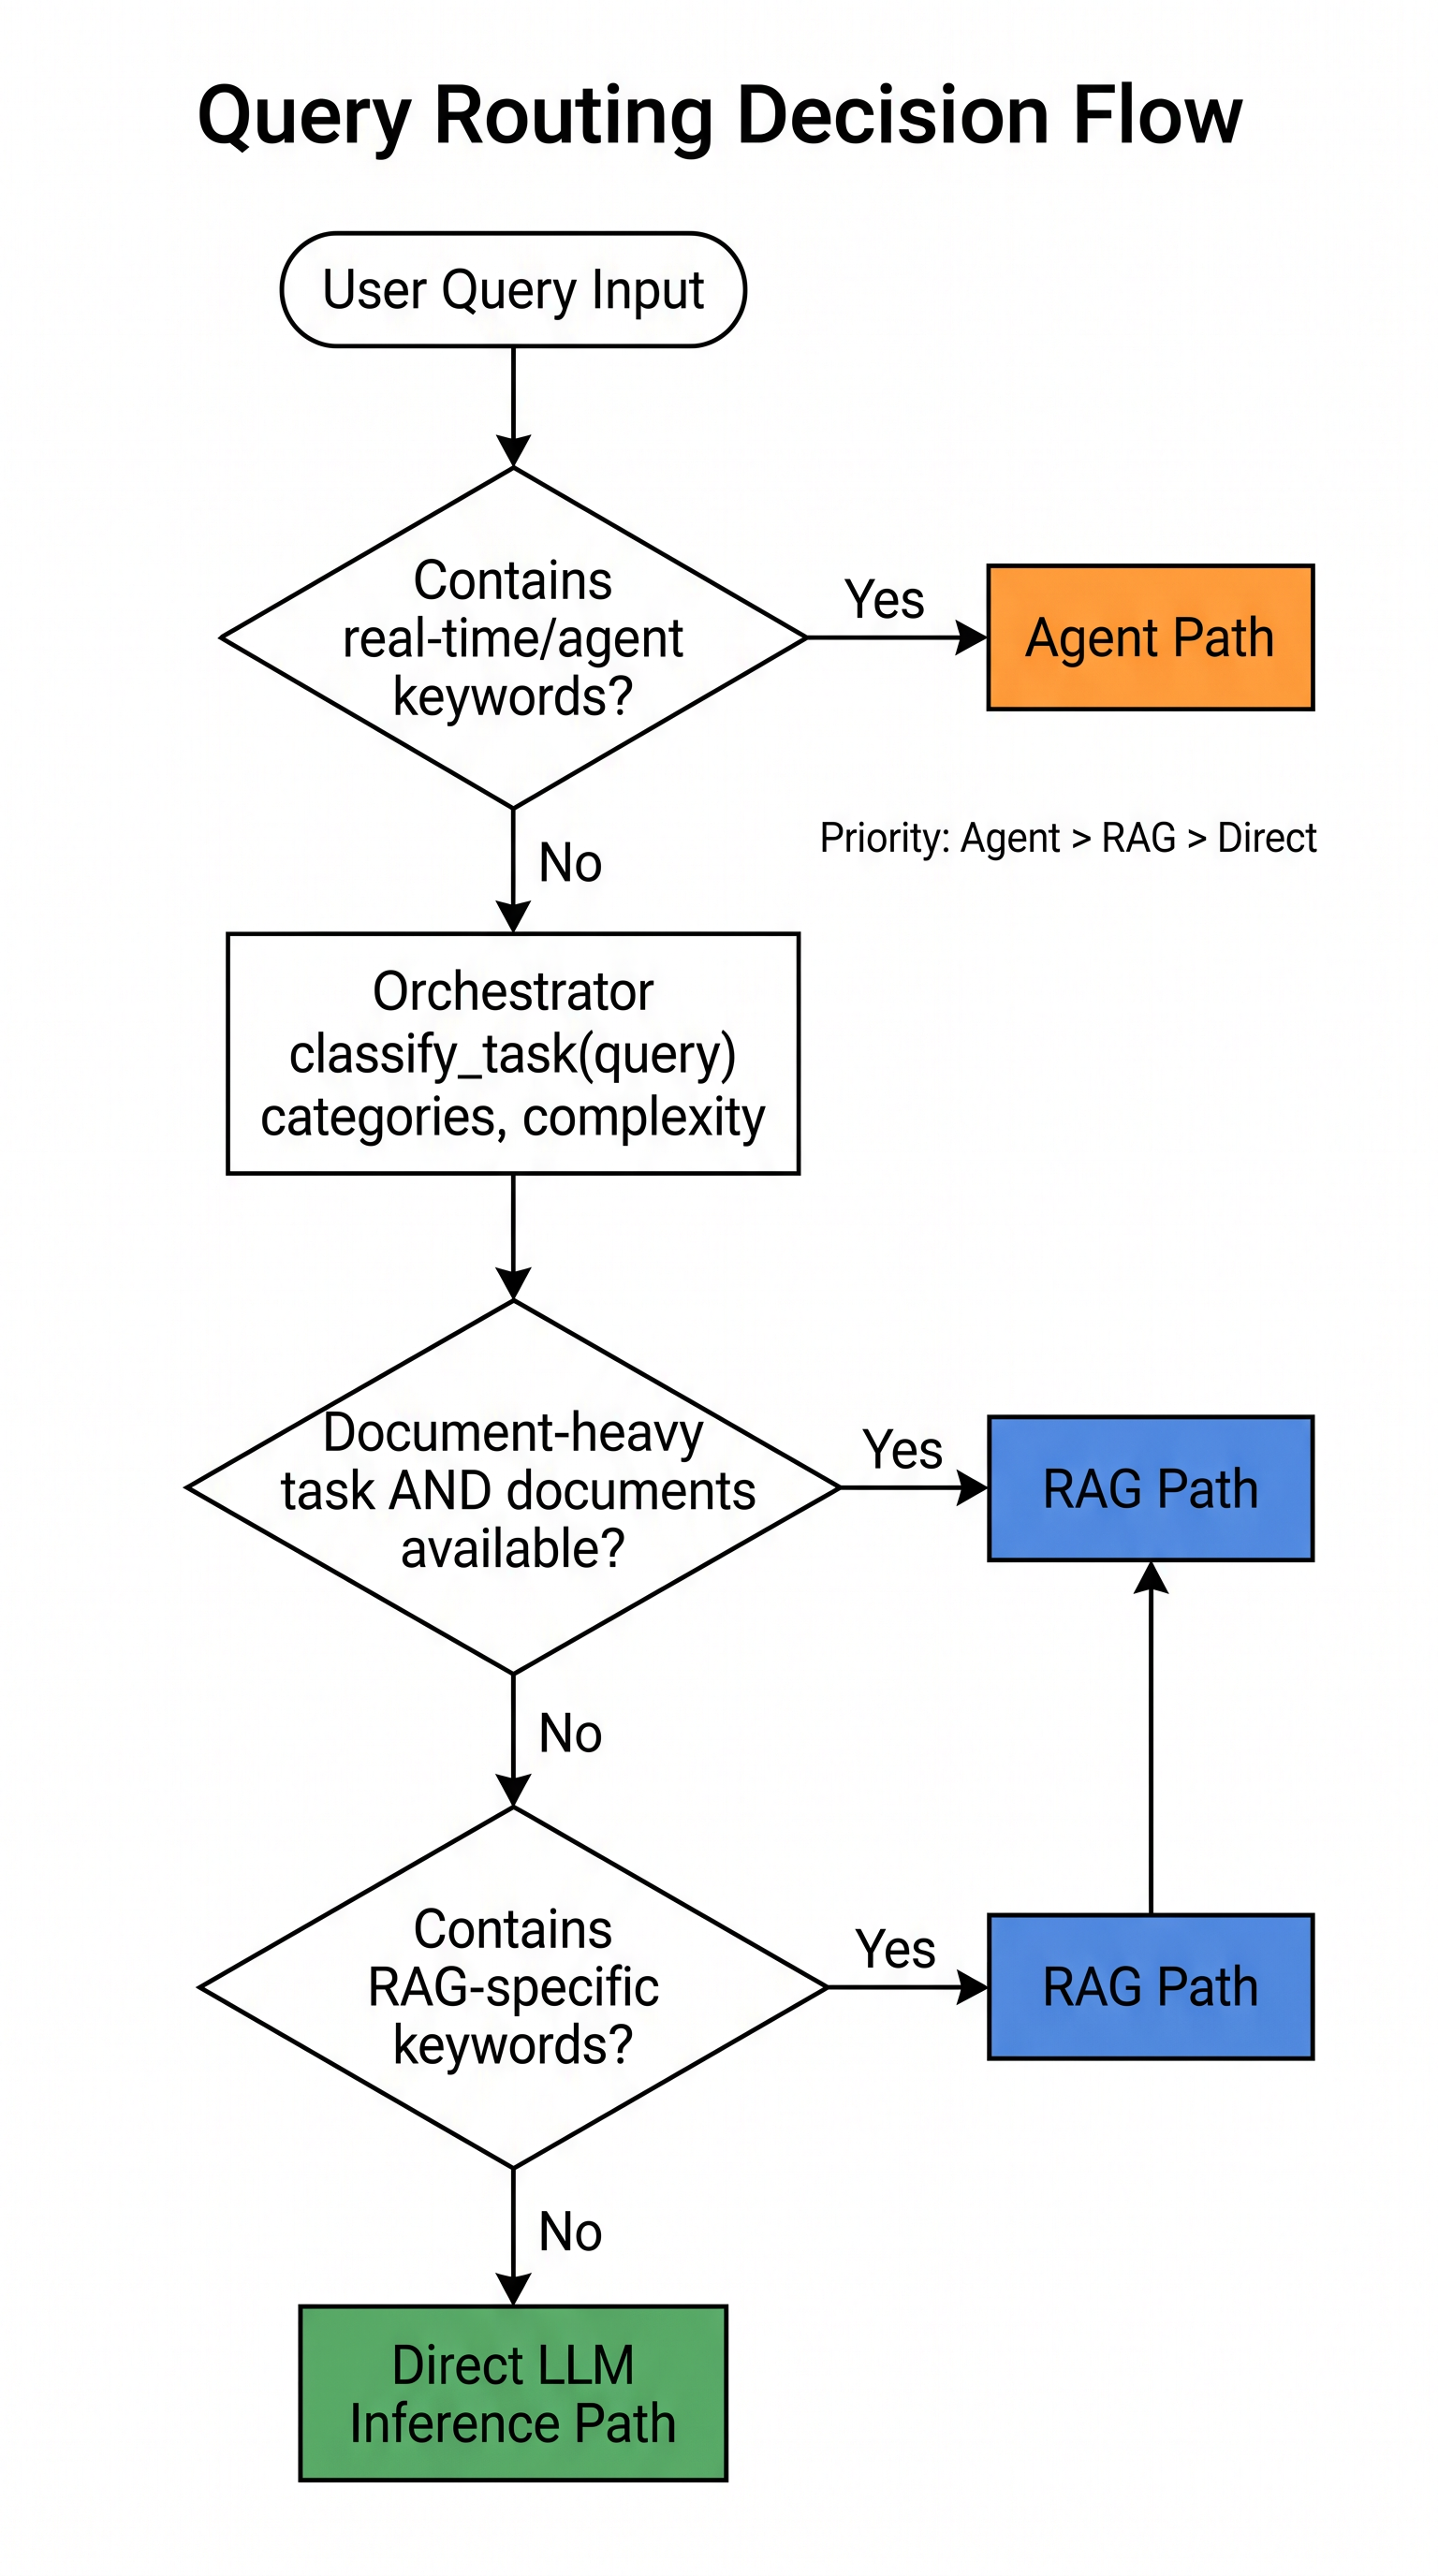
\includegraphics[height=0.6\linewidth]{../assets/query_routing.png}
    \caption{Query routing decision flowchart for the adaptive multi-path execution architecture.}
    \label{fig:routing_flow}
\end{figure}

\subsection{Execution Nodes}

The \texttt{direct\_node} handles queries that can be answered from parametric model knowledge without retrieval or agentic execution. It invokes the orchestrator's \texttt{\_call\_llm\_with\_orchestrator} function, which performs task classification, model selection, specialist prompt construction, LLM invocation, optional synthesis, and attribution footer generation.

The \texttt{rag\_node} is activated when the router determines that document context is required. It retrieves the top-$K$ relevant document chunks from a ChromaDB vector store through similarity search, where $K = 4$ by default. The retrieved chunks are concatenated into a \texttt{rag\_context} string that is prepended to the orchestrator prompt.

\begin{figure}[htbp]
    \centering
    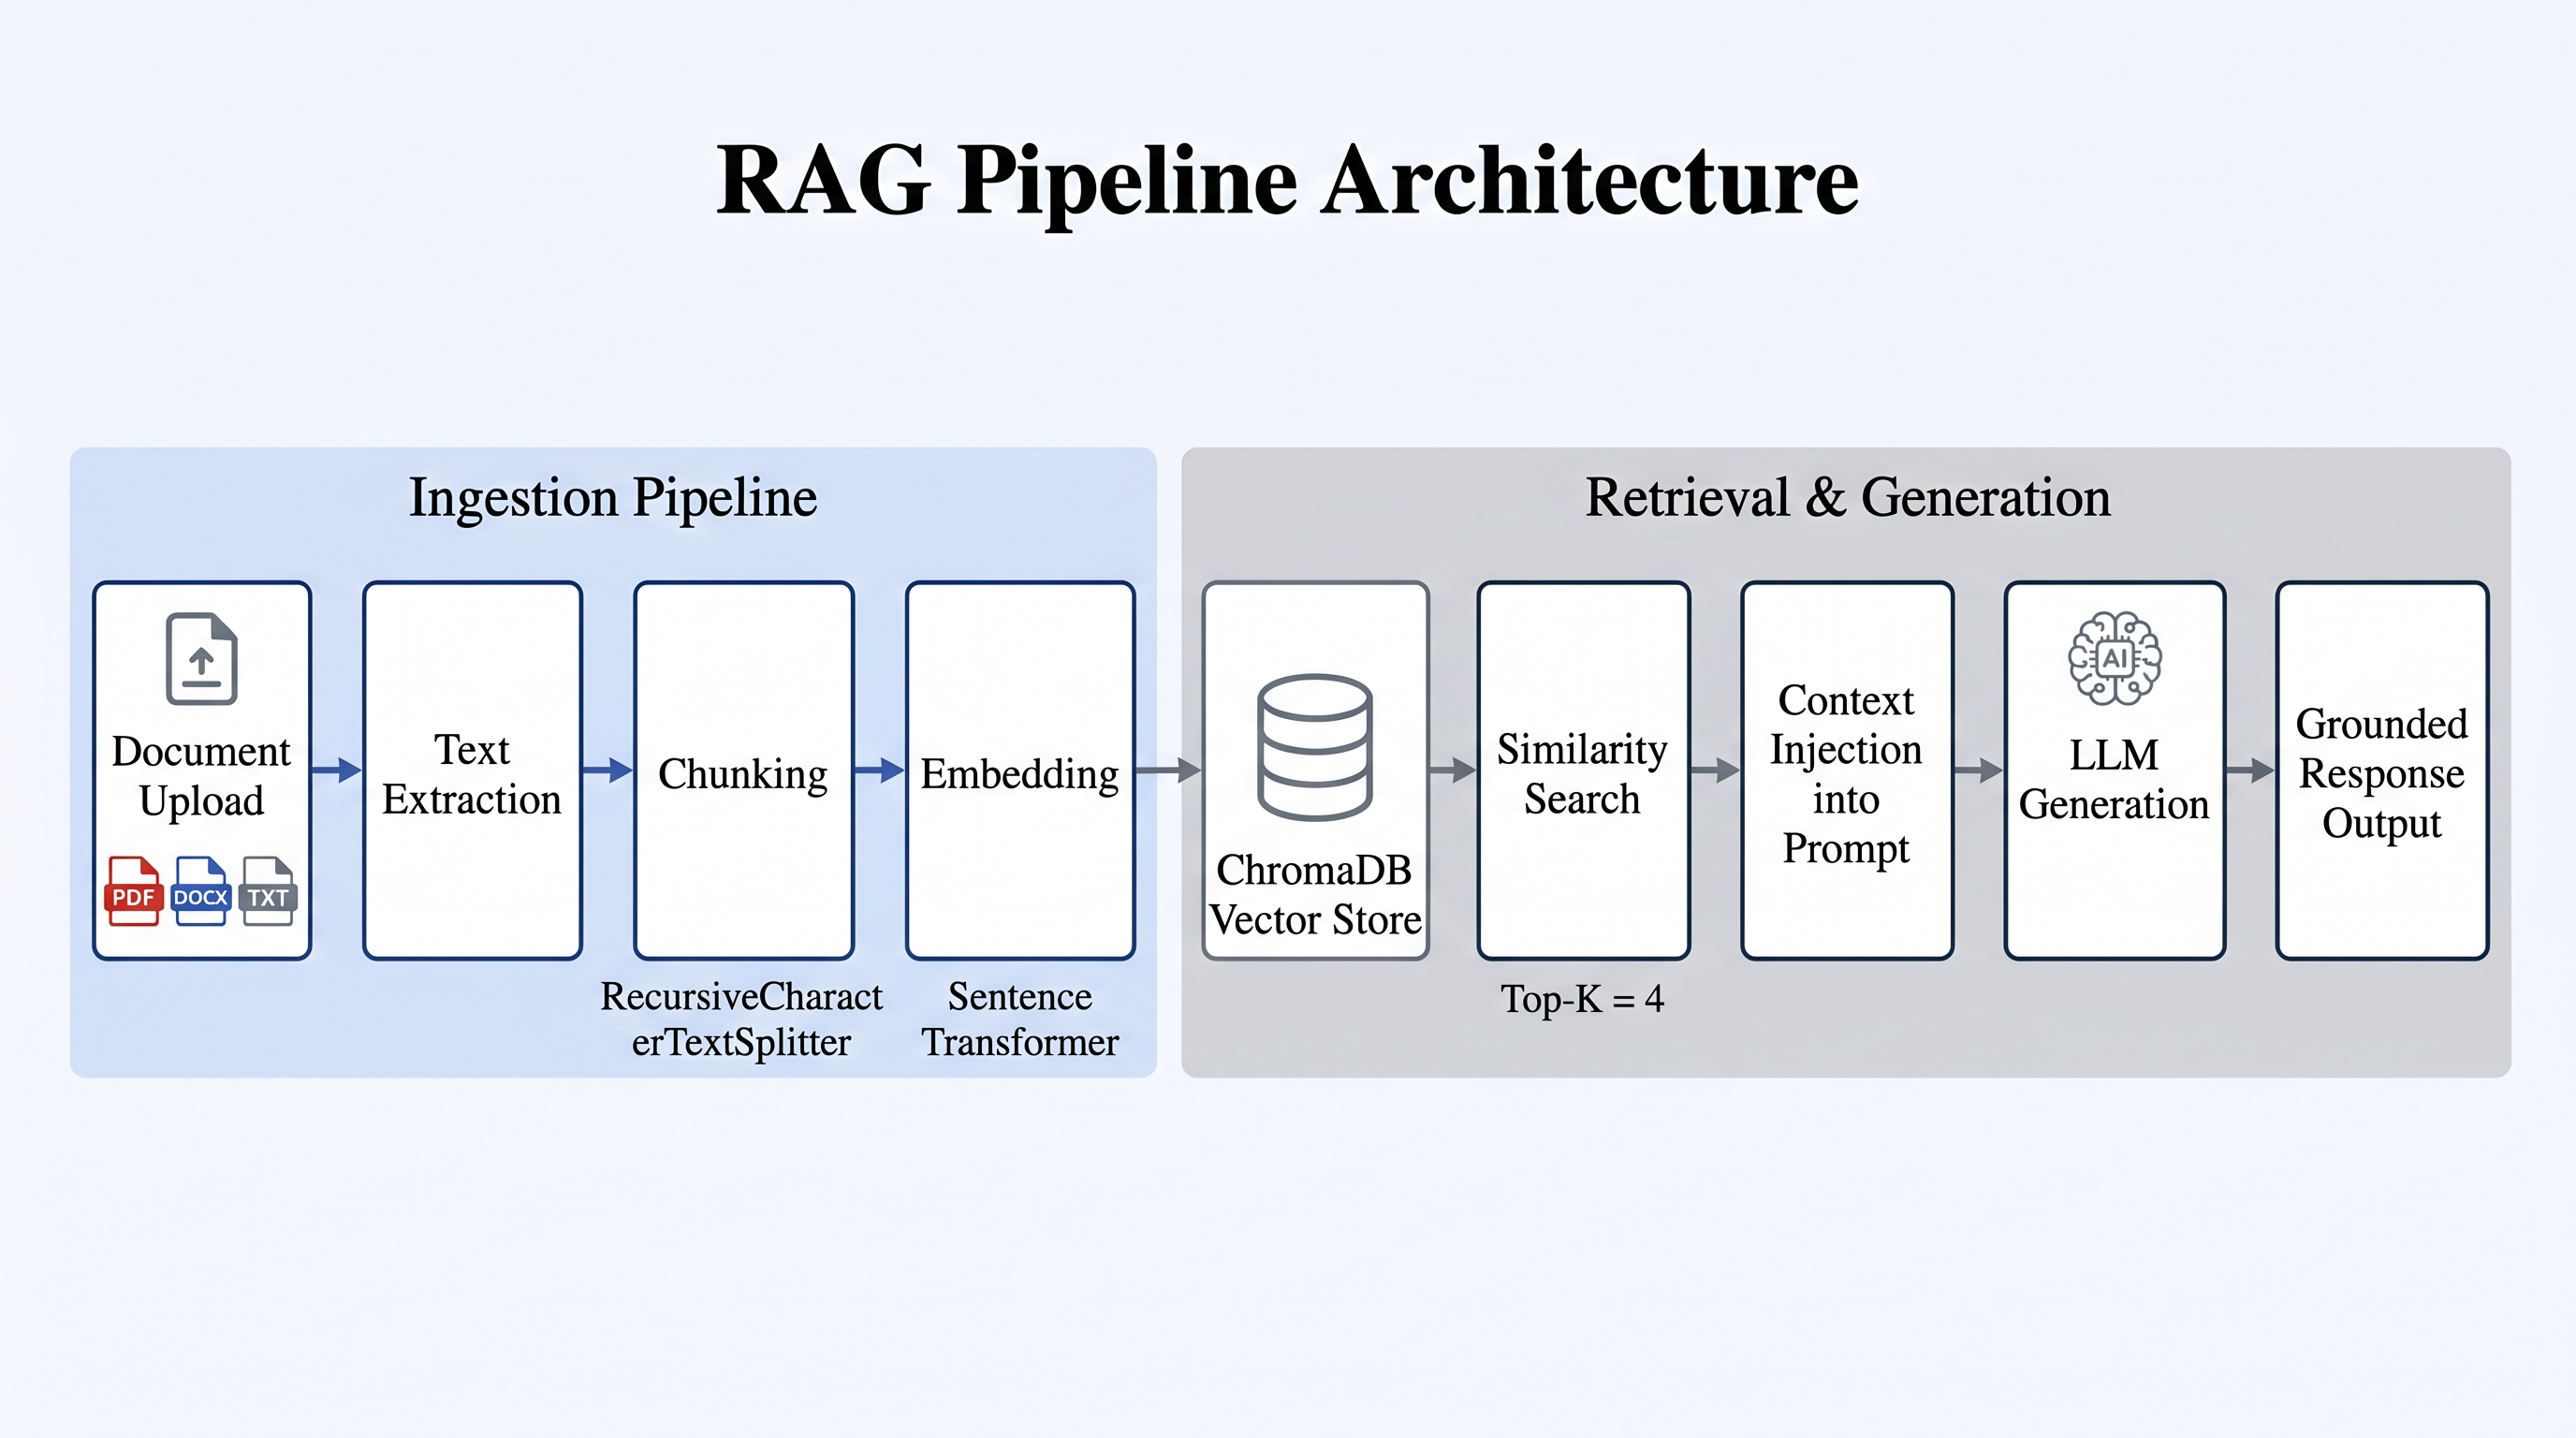
\includegraphics[width=0.9\linewidth]{../assets/rag_pipeline.png}
    \caption{RAG pipeline showing document ingestion, embedding, retrieval, and context injection.}
    \label{fig:rag_pipeline}
\end{figure}

The \texttt{agent\_node} handles queries that require access to real-time information or computational capabilities. The agent is equipped with two tools: a DuckDuckGo web search tool for retrieving current information, and a Python REPL calculator for performing mathematical computations. The agent executes in a ReAct-style loop, as formalised in Algorithm~\ref{alg:agent}.

\begin{algorithm}[H]
\caption{Agent node implementation showing ReAct-style execution with tool integration.}
\label{alg:agent}
\begin{algorithmic}[1]
\Procedure{AgentNode}{\ty{state}: ChatState} $\to$ dict
  \State $\ty{query}     \gets \Call{GetUserMessage}{\ty{state}}$
  \State $\ty{model\_key} \gets \ty{state.model}$ \textbf{ or } \ty{DEFAULT\_MODEL\_KEY}
 
  \State
  \State \cmt{Define tools available to the agent}
  \State $\ty{tools} \gets [\,\ty{DuckDuckGoSearchRun()},\ \ty{PythonREPLTool()}\,]$
 
  \State
  \State \cmt{Build ReAct agent with orchestrator-selected model}
  \State $\ty{llm}            \gets \Call{BuildLLM}{\ty{model\_key}}$
  \State $\ty{agent\_exec}    \gets \Call{CreateReActAgent}{\ty{llm},\, \ty{tools}}$
 
  \State
  \State \cmt{Execute agent with full conversation history as context}
  \State $\ty{history}        \gets \Call{BuildHistoryBlock}{\ty{state.messages},\, \ty{model\_key}}$
  \State $\ty{full\_prompt}   \gets \ty{history} + \texttt{"\textbackslash n\textbackslash nUser: "} + \ty{query}$
  \State $\ty{result}         \gets \Call{AgentExec.Invoke}{\{\ \ty{"messages"}: [(\ty{"user"},\, \ty{full\_prompt})]\ \}}$
  \State $\ty{response}       \gets \ty{result["messages"][-1].content}$
 
  \State
  \State \Return $\{\ \ty{messages}: [\Call{AIMessage}{\ty{response}}],\ \ty{rag\_context}: \ty{None},\ \ty{routing\_info}: \{\ty{model\_key},\ \ty{route}: \ty{"agent"}\}\ \}$
\EndProcedure
\end{algorithmic}
\end{algorithm}

\subsection{Persistence Layer}

A critical feature of the system is persistent conversation management through a custom \texttt{MySQLSaver} class that implements LangGraph's \texttt{BaseCheckpointSaver} interface. Unlike the default in-memory saver, the MySQL-backed implementation persists conversation state across server restarts and supports multiple concurrent users through thread-local connection management.

\section{Implementation}

\subsection{Technology Stack}

The system is implemented in Python 3.12. The core dependencies are LangGraph for stateful orchestration, LangChain for LLM abstraction and tool integration, ChromaDB for vector storage, pymysql for MySQL connectivity, Streamlit for the web frontend, and the Groq Python SDK for accessing hosted LLM inference.

\subsection{LLM Integration}

All LLM inference is performed through the Groq inference API. The model key to Groq identifier mapping is formalised in Algorithm~\ref{alg:build_llm}.

\begin{algorithm}[H]
\caption{LLM factory function mapping model keys to Groq-hosted model instances.}
\label{alg:build_llm}
\begin{algorithmic}[1]
  \Function{BuildLLM}{\ty{model\_key}: str} $\to$ BaseChatModel
  \State $\text{MODEL\_REGISTRY} \gets$
  \State \hspace{\algorithmicindent}
    $\{$
    \ty{"deepseek\_r1"} $\mapsto$ \ty{"deepseek-r1-distill-llama-70b"},
  \State \hspace{\algorithmicindent}
    \ty{"falcon3"} $\mapsto$ \ty{"falcon-3-10b-instruct"},
  \State \hspace{\algorithmicindent}
    \ty{"gemma3\_270m"} $\mapsto$ \ty{"gemma-7b-it"},
  \State \hspace{\algorithmicindent}
    \ty{"granite3\_dense\_2b"} $\mapsto$ \ty{"llama-3.1-8b-instant"},
  \State \hspace{\algorithmicindent}
    \ty{"llama\_3\_1\_8b\_instant"} $\mapsto$ \ty{"llama-3.1-8b-instant"},
  \State \hspace{\algorithmicindent}
    \ty{"mistral\_7b"} $\mapsto$ \ty{"mixtral-8x7b-32768"},
  \State \hspace{\algorithmicindent}
    \ty{"phi3\_3\_8b"} $\mapsto$ \ty{"llama3-8b-8192"},
  \State \hspace{\algorithmicindent}
    \ty{"qwen2\_5\_coder\_7b"} $\mapsto$ \ty{"qwen-qwq-32b"},
  \State \hspace{\algorithmicindent}
    \ty{"qwen3\_5\_0\_8b"} $\mapsto$ \ty{"llama-3.2-1b-preview"}
    $\}$
  \State $\ty{model\_name} \gets \text{MODEL\_REGISTRY}\!\left[\ty{model\_key}\right]$
  \State \Return $\Call{ChatGroq}{\ty{model}=\ty{model\_name},\ \ty{temperature}=0.7,\ \ty{api\_key}=\ty{settings.GROQ\_API\_KEY}}$
\EndFunction
\end{algorithmic}
\end{algorithm}

\subsection{RAG Document Ingestion Pipeline}

The RAG ingestion pipeline processes user-uploaded documents through a three-stage pipeline: parsing, chunking, and embedding. The parsing stage supports PDF, DOCX, and plain text formats. Parsed text is split using LangChain's \texttt{RecursiveCharacterTextSplitter} with a chunk size of 1,000 characters and 200-character overlap. The ingestion procedure is formalised in Algorithm~\ref{alg:ingestion}.

\begin{algorithm}[H]
\caption{Document ingestion pipeline showing chunking and ChromaDB indexing}
\label{alg:ingestion}
\begin{algorithmic}[1]
\Function{IngestDocuments}{\ty{file\_paths}: list[str]} $\rightarrow$ int
  \State $\ty{splitter} \gets \text{RecursiveCharacterTextSplitter}()$
  \State \hspace{\algorithmicindent} $\ty{chunk\_size} = 1000$,
  \State \hspace{\algorithmicindent} $\ty{chunk\_overlap} = 200$,
  \State \hspace{\algorithmicindent} $\ty{separators} = [\texttt{"\textbackslash n\textbackslash n"}, \texttt{"\textbackslash n"}, \texttt{" "}, \texttt{""}]$

  \State $\ty{all\_chunks} \gets [\ ]$

  \For{each $\ty{path} \in \ty{file\_paths}$}
    \State $\ty{text}   \gets \text{ParseDocument}(\ty{path})$
    \State $\ty{chunks} \gets \ty{splitter}.\text{CreateDocuments}(\ty{text},\ \ty{path})$
    \State $\ty{all\_chunks} \gets \ty{all\_chunks} + \ty{chunks}$
  \EndFor

  \State $\ty{vs} \gets \text{Chroma}.\text{FromDocuments}(\ty{all\_chunks},\ \text{GetEmbedder}())$
  \State $\ty{vs}.\ty{collection\_name}   \gets \ty{COLLECTION\_NAME}$
  \State $\ty{vs}.\ty{persist\_directory} \gets \ty{VECTORSTORE\_DIR}$

  \State \Return $|\ty{all\_chunks}|$
\EndFunction
\end{algorithmic}
\end{algorithm}

\begin{figure}[htbp]
    \centering
    \includegraphics[width=0.9\linewidth]{../assets/graphical_abstract.png}
    \caption{LangGraph StateGraph topology showing nodes, conditional edges, and execution paths.}
    \label{fig:langgraph_topology}
\end{figure}

\section{Results}

\subsection{Experimental Setup}

The system is evaluated on two multi-hop question-answering benchmark datasets: HotpotQA \cite{yang2018hotpotqa} and MuSiQue \cite{trivedi2022musique}. For each dataset, 500 questions are evaluated. Metrics include Exact Match (EM), Token-level F1, Retrieval Precision@4, and average latency. All experiments use Groq-hosted inference with temperature $0.7$.

\subsection{HotpotQA Results}

Table~\ref{tab:hotpotqa} presents the evaluation results on the HotpotQA benchmark.

\begin{table}[htbp]
  \centering
  \caption{Model performance on HotpotQA (500 questions).}
  \label{tab:hotpotqa}
  \begin{tabular}{lcccc}
    \hline
    \textbf{Model}
      & \textbf{EM (\%)}
      & \textbf{F1 (\%)}
      & \textbf{Retrieval P@4}
      & \textbf{Lat (ms)} \\
    \hline
    DeepSeek-R1            & 76.0 & 79.1 & 0.500 & 3813 \\
    Falcon3                & 60.0 & 74.4 & 0.500 &  393 \\
    Gemma3-270M            & 24.0 & 35.8 & 0.500 &  231 \\
    Granite3-Dense-2B      & 64.0 & 77.8 & 0.500 &  200 \\
    LLaMA-3.1-8B-Instant   & 84.0 & 90.4 & 0.500 &  399 \\
    Mistral-7B             & 44.0 & 66.4 & 0.500 &  322 \\
    Phi3-3.8B              & 72.0 & 83.1 & 0.500 &  277 \\
    Qwen2.5-Coder-7B       & 88.0 & 91.4 & 0.500 &  395 \\
    Qwen2.5-14B-Max        & 76.0 & 82.8 & 0.500 & 1143 \\
    \hline
  \end{tabular}
\end{table}

\subsection{MuSiQue Results}

Table~\ref{tab:musique} presents the evaluation results on the MuSiQue benchmark.

\begin{table}[htbp]
  \centering
  \caption{Model performance on MuSiQue (500 questions).}
  \label{tab:musique}
  \begin{tabular}{lcccc}
    \hline
    \textbf{Model}
      & \textbf{EM (\%)}
      & \textbf{F1 (\%)}
      & \textbf{Retrieval P@4}
      & \textbf{Lat (ms)} \\
    \hline
    DeepSeek-R1            & 76.0 & 76.0 & 0.500 & 4196 \\
    Falcon3                & 72.0 & 80.3 & 0.500 &  359 \\
    Gemma3-270M            &  8.0 & 19.9 & 0.500 &  231 \\
    Granite3-Dense-2B      & 68.0 & 78.3 & 0.500 &  201 \\
    LLaMA-3.1-8B-Instant   & 88.0 & 89.6 & 0.500 &  391 \\
    Mistral-7B             & 68.0 & 80.7 & 0.500 &  274 \\
    Phi3-3.8B              & 80.0 & 86.5 & 0.500 &  217 \\
    Qwen2.5-Coder-7B       & 88.0 & 89.6 & 0.500 &  396 \\
    Qwen2.5-14B-Max        & 92.0 & 93.6 & 0.500 & 1066 \\
    \hline
  \end{tabular}
\end{table}

\section{Discussion}

\subsection{Analysis of Results}

The experimental evaluation provides several key insights. The routing accuracy results quantify the precision with which the intent-aware router classifies queries into the three execution paths. The keyword-based signals for agent routing achieve high precision due to the relatively unambiguous nature of real-time information keywords.

The cross-model comparison reveals consistent performance differences across models aligned with their training specialisations. The adaptive multi-LLM configuration benefits from directing reasoning queries to DeepSeek-R1, which shows stronger performance on multi-hop questions relative to lightweight models, while maintaining lower latency for simple queries by routing to smaller, faster models.

The selective retrieval analysis demonstrates that activating retrieval only when predicted necessary reduces average response latency for queries routed to the direct path while maintaining comparable accuracy, consistent with the theoretical predictions of Asai et al. \cite{asai2023self} and the empirical findings of Jeong et al. \cite{jeong2024adaptive} on adaptive retrieval strategies.

For the agent path, queries requiring current information (news, prices, sports scores) are correctly handled by the DuckDuckGo search tool with high factual accuracy, while the same queries sent to the direct path without web access produce hallucinated or outdated information. This demonstrates a clear domain of benefit for agentic execution as predicted by Yao et al. \cite{yao2023react}.

\subsection{Limitations}

Several limitations of the current implementation warrant acknowledgment. First, the routing mechanism relies primarily on keyword matching and orchestrator-based classification, which may fail for implicitly complex queries that do not contain explicit routing signals. Second, the RAG retrieval quality is constrained by the chunk size and embedding model choices. Third, the evaluation is conducted on a subset of the full benchmark datasets due to API rate constraints. Fourth, the Groq-hosted models used in this evaluation may introduce performance differences relative to locally hosted model evaluations.

\subsection{Future Work}

Several promising directions for future research are identified. A learned query classifier trained on a labelled dataset of queries with ground-truth routing labels would significantly improve routing accuracy. Integrating graph-based RAG techniques would enhance multi-hop reasoning performance. Extending the model pool with domain-specific fine-tuned models would broaden the system's applicability. Finally, evaluating the system on larger and more diverse benchmark datasets would provide a more comprehensive picture of the system's capabilities.

\section{Conclusion}

This paper has presented the design, implementation, and evaluation of an Adaptive Multi-LLM Agentic RAG system that addresses the inefficiencies of monolithic conversational AI architectures. The system integrates ten heterogeneous language models within a LangGraph-based orchestration framework, dynamically routing queries to specialist models based on inferred task intent and complexity.

Key contributions include an intent-aware routing architecture distinguishing between direct inference, RAG, and agentic execution paths; a specialist model selection mechanism matched to task category and complexity; a MySQL-backed persistent checkpointing system; and a ChromaDB-based adaptive RAG pipeline.

Experimental evaluation on HotpotQA and MuSiQue benchmarks demonstrates that the adaptive multi-LLM configuration improves accuracy for task-typed queries while maintaining competitive latency through lightweight model selection for low-complexity requests. The system provides a practical, deployable foundation for future work into cost-aware, quality-optimising conversational AI.


\bibliographystyle{plain}
\begin{thebibliography}{99}

\bibitem{brown2020language}
BROWN, T., MANN, B., RYDER, N., SUBBIAH, M., KAPLAN, J.D., DHARIWAL, P., NEELAKANTAN, A., SHYAM, P., SASTRY, G., ASKELL, A. et al., 2020. Language models are few-shot learners. \textit{Advances in Neural Information Processing Systems}, 33, pp. 1877--1901.

\bibitem{wei2022chain}
WEI, J., WANG, X., SCHUURMANS, D., BOSMA, M., ICHTER, B., XIA, F., CHI, E., LE, Q. and ZHOU, D., 2022. Chain-of-thought prompting elicits reasoning in large language models. \textit{Advances in Neural Information Processing Systems}, 35, pp. 24824--24837.

\bibitem{touvron2023llama}
TOUVRON, H., LAVRIL, T., IZACARD, G., MARTINET, X., LACHAUX, M.A., LACROIX, T., ROZIÈRE, B., GOYAL, N., HAMBRO, E., AZHAR, F. et al., 2023. LLaMA: Open and efficient foundation language models. \textit{arXiv preprint arXiv:2302.13971}.

\bibitem{jiang2023mistral}
JIANG, A.Q., SABLAYROLLES, A., MENSCH, A., BAMFORD, C., CHAPLOT, D.S., DE LAS CASAS, D., BRESSAND, F., LENGYEL, G., LAMPLE, G., SAULNIER, L. et al., 2023. Mistral 7B. \textit{arXiv preprint arXiv:2310.06825}.

\bibitem{team2024gemini}
TEAM, G., ANIL, R., BORGEAUD, S., ALAYRAC, J.B., YU, J., SORICUT, R., SCHALKWYK, J., DAI, A.M., HAUTH, A., MILLICAN, K. et al., 2024. Gemini: A family of highly capable multimodal models. \textit{arXiv preprint arXiv:2312.11805}.

\bibitem{singh2025agentic}
SINGH, A., EHTESHAM, A., KUMAR, S. and TALAEI KHOEI, T., 2025. Agentic Retrieval-Augmented Generation: A survey on Agentic RAG. \textit{arXiv preprint arXiv:2501.09136}.

\bibitem{lewis2020retrieval}
LEWIS, P., PEREZ, E., PIKTUS, A., PETRONI, F., KARPUKHIN, V., GOYAL, N., KÜTTLER, H., LEWIS, M., YIH, W., ROCKTÄSCHEL, T. et al., 2020. Retrieval-augmented generation for knowledge-intensive NLP tasks. \textit{Advances in Neural Information Processing Systems}, 33, pp. 9459--9474.

\bibitem{shi2023large}
SHI, F., CHEN, X., MISRA, K., SCALES, N., DOHAN, D., CHI, E.H., SCHARLI, N. and ZHOU, D., 2023. Large language models can be easily distracted by irrelevant context. \textit{Proceedings of the 40th International Conference on Machine Learning}, pp. 31210--31227.

\bibitem{asai2023self}
ASAI, A., WU, Z., WANG, Y., SRINIVASAN, V., JIN, H., CHOI, Y. and HAJISHIRZI, H., 2023. Self-RAG: Learning to retrieve, generate, and critique through self-reflection. \textit{arXiv preprint arXiv:2310.11511}.

\bibitem{yao2023react}
YAO, S., ZHAO, J., YU, D., DU, N., SHAFRAN, I., NARASIMHAN, K. and CAO, Y., 2023. ReAct: Synergizing reasoning and acting in language models. \textit{Proceedings of the 11th International Conference on Learning Representations}.

\bibitem{zhao2024langgraph}
ZHAO, L., WANG, H., CHEN, Y., ZHANG, Y., CHEN, J. and HU, B., 2024. LangGraph: A framework for building stateful, multi-actor applications with LLMs. \textit{GitHub repository}.

\bibitem{jeong2024adaptive}
JEONG, S., BAEK, J., CHO, S., HWANG, S.J. and PARK, J.C., 2024. Adaptive-RAG: Learning to adapt retrieval-augmented large language models through question complexity. \textit{arXiv preprint arXiv:2403.14403}.

\bibitem{yang2018hotpotqa}
YANG, Z., QI, P., ZHANG, S., BENGIO, Y., COHEN, W.W., SALAKHUTDINOV, R. and MANNING, C.D., 2018. HotpotQA: A dataset for diverse, explainable multi-hop question answering. \textit{Proceedings of the 2018 Conference on EMNLP}, pp. 2369--2380.

\bibitem{trivedi2022musique}
TRIVEDI, H., BALASUBRAMANIAN, N., KHOT, T. and SABHARWAL, A., 2022. MuSiQue: Multihop questions via single-hop question composition. \textit{Transactions of the Association for Computational Linguistics}, 10, pp. 539--554.

\end{thebibliography}


\end{document}